\chapter{Implementation}
\label{chapter:implementation}

In this section there is a description of the implemented solution: hardware in the \autoref{sec:impl_hardware}, used software tools in the \autoref{sec:impl_software} and integration of all parts together in the \autoref{sec:impl_integration}. The code can be found on GitHub: stereo pair driver\footnote{\url{https://github.com/Myralllka/UAV_basler_stereopair_driver}} and the main module\footnote{\url{https://github.com/Myralllka/UAV_localisation_from_cameras}}.

\section{Hardware}
\label{sec:impl_hardware}
\begin{figure}[h]
  \begin{subfigure}[b]{0.49\textwidth}
    \centering
    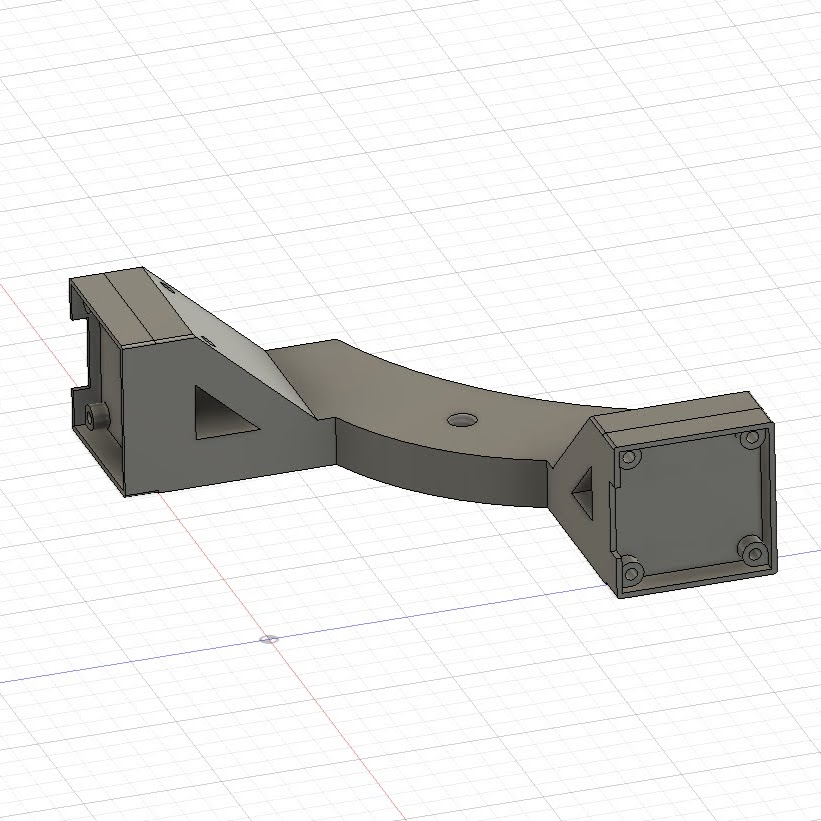
\includegraphics[width=\textwidth]{graphics/CAD.jpg}
    \caption{The CAD model of the prototype}
    \label{fig:proto_scheme}
  \end{subfigure}
  \hfill
  \begin{subfigure}[b]{0.49\textwidth}
    \centering
    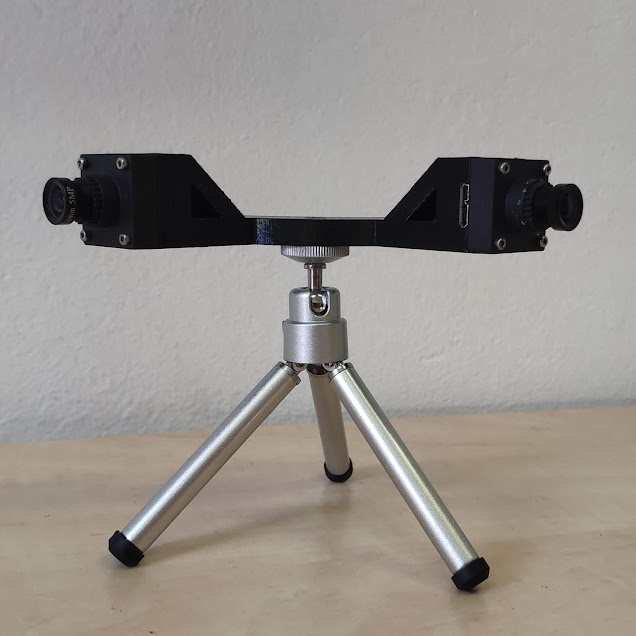
\includegraphics[width=\textwidth]{graphics/prototype.jpg}
    \caption{The printed prototype}
    \label{fig:proto_printed}
  \end{subfigure}
  \label{The proposed sollution prototype}
\end{figure}

The camera holder CAD model was created in a Fusion360 software considering requirements of rotation $90^\circ$ and the distance close to the average MAV sizes, the screenshot from the modelling process is in \autoref{fig:proto_scheme}.
The 3d-printed solution prototype with cameras mounted is in the \autoref{fig:proto_printed}

Basler daA1600-60um cameras were chosen for this project because they have a global shutter to capture moving objects, good image quality and they are not so expensive.
\begin{center}
    \begin{tabular}{ l l }
    \hline
    name                   & property          \\ \hline
    Lens mount type        & S-mount           \\
    Data transfer protocol & USB 3.0           \\
    Max. frame rate        & 60 fps            \\
    Resolution (HxV)       & 1600 px x 1200 px \\
    Resolution             & 2 MP              \\
    Price                  & 289.00 EUR        \\ \hline
    \end{tabular}
\end{center}

Cameras' lences have $120^\circ$ FOV, which gives enough overlapping zone to detect features in $\sigma$ (see \autoref{fig:sch_stereo}).

Intel NUC with 8 cores CPU is used as the onboard computer for MAV. 
No external GPU is needed, so all algorithms should consider it.

\section{Software tools}
\label{sec:impl_software}

The proposed solution uses the Robotic operating system (ROS)\cite{Rospaper} as the middleware.
ROS is the whole ecosystem with hundreds of already implemented algorithms and libraries to interact with robots between Its parts and sensors.
It is an open-source tool, so the apriltag detector and camera driver used in this thesis are based on official modules from the ROS community.

The MRS UAV system \cite{Baca2021} is used as a drone control environment. It is based on ROS, but it is the unique framework for MAVs to implement and test path planning, control, computer vision, object tracking, and many more MAV-related problems.

OpenCV \cite{opencv} is an open-source library for computer vision.
Eigen \cite{Eigen} is an efficient library for linear algebra.
Some solution algorithm implementations were used in both of them.

\section{Integration}
\label{sec:impl_integration}

Implementation steps are described in the same order as in a \autoref{chapter:methodology}: calibrations, features matching, extracting 3D poses of features, and error computation.

\begin{figure}[h]
    \centering
    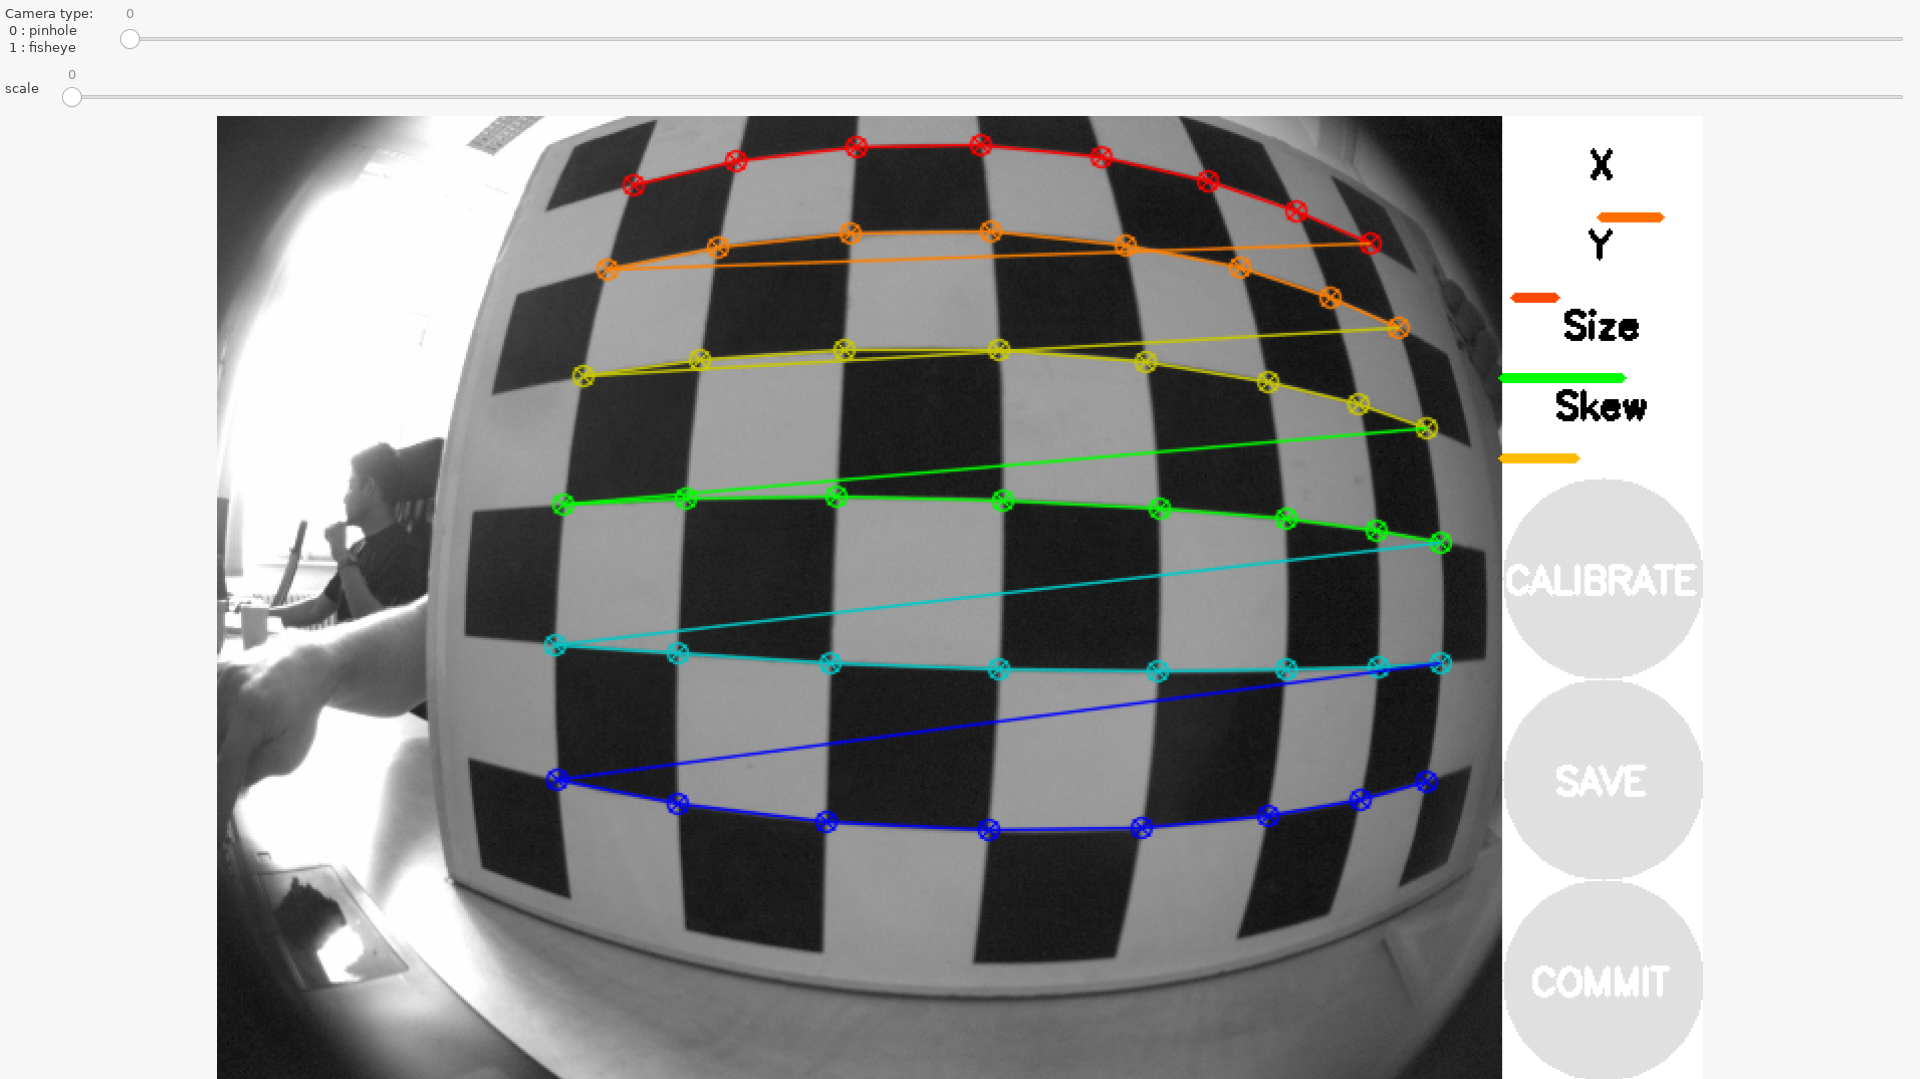
\includegraphics[width=.6\textwidth]{graphics/calibration.png}
    \caption{The calibration process}
    \label{fig:calib}
\end{figure}

There is a package\footnote{\url{http://wiki.ros.org/camera_calibration}} in ROS ecosystem, that was used for the camera calibration process described in \autoref{sec:meth_calib}. 
It takes a chessboard parameter (square size and the number of squares) as input.
Then in the interactive mode (see \autoref{fig:calib}), it collects images for calibration and, as a result, creates a file with the camera calibration matrix and distortion coefficients if the lens has it.

There are two implemented methods of stereo pair calibration described in \autoref{sec:stereocalib}.
Both of them use an apriltag calibration pattern, shown in the \autoref{fig:aptags}.
The main reason why this pattern was chosen is that each tag can be detected individually, so there is no need to have all of them simultaneously in the overlapping zone.
The first method is implemented using the "Least-square estimation of transformation between two point sets" \cite{Umeyama1991} implementation from Eigen.
As the initial poses, measurements from the CAD model are used.
The second method is implemented using the OpenCV PnP solver.
As far as a standard apriltag detector outputs only the 3D poses of detected tags, it was modified to publish external information needed for the PnP algorithm - 2D coordinates of apriltags' corners in each image.

After both cameras and stereo pair are calibrated, the following steps are features detection, matching and filtering (\autoref{sec:features}) for a synchronized pair of images. 
The synchronization is done on the stereo pair driver level.

As described in \autoref{sec:features}, ORB detector and brute-force matcher from OpenCV were used for features detection and matching.
Even after this process, there will be some outliers.
Distance from features to the corresponding epipolar lines can be used to filter them. 
This distance can be computed using the equation \autoref{eq:epiconstr}.
Its result is $0$ only in an ideal case; otherwise, the equation result will be the distance from the reprojected point to its corresponding epipolar line.

The next step is to reconstruct the 3D scene from obtained feature points.
There are two different methods implemented for that, described in \autoref{sec:svdtriang} and \autoref{sec:shortest_distance}.
One of them is an algebraic solution of the shortest distance between two rays, so it completely depends on calibration quality.
Another one is called "The Golden Standard Triangulation Method", which combines SVD triangulation with applied Sampson correction. 
The implementation from the OpenCV is used.

As a result, obstacles in the cameras' overlapping zone are detected in a format of the point cloud and correspondent feature points on both images.
Recalling the \autoref{fig:intro_general}, the proposed solution providing a pointcloud with obstacles in a red zone at each timestamp $t_i$. 
